\chapter{Implementation}
\label{cha:implementation}

\section{Work plan --- Work packages, deliverables}
\label{sec:work-plan}

\subsection{Overall structure}
\label{sec:wpstructure}

\begin{figure}
    \centering
    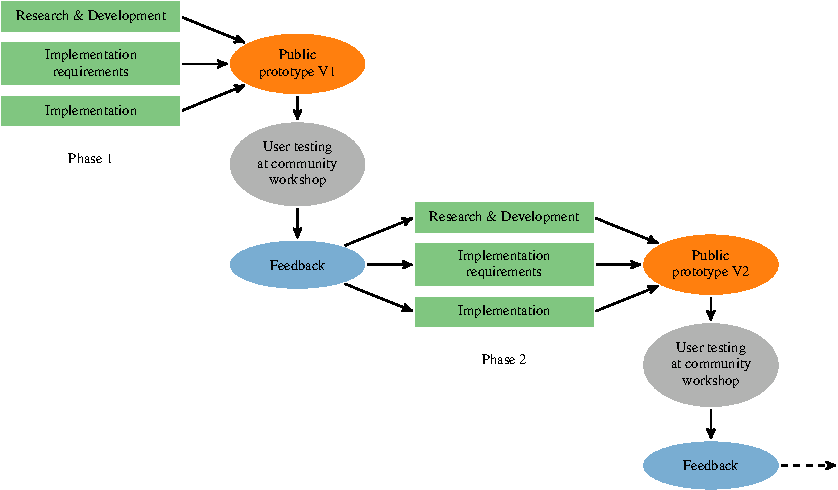
\includegraphics[width=\linewidth]{workflow.pdf}
    \caption{Iterative workflow for {\acro}.}
    \label{fig:workflow}
\end{figure}

\begin{figure}
    \centering
    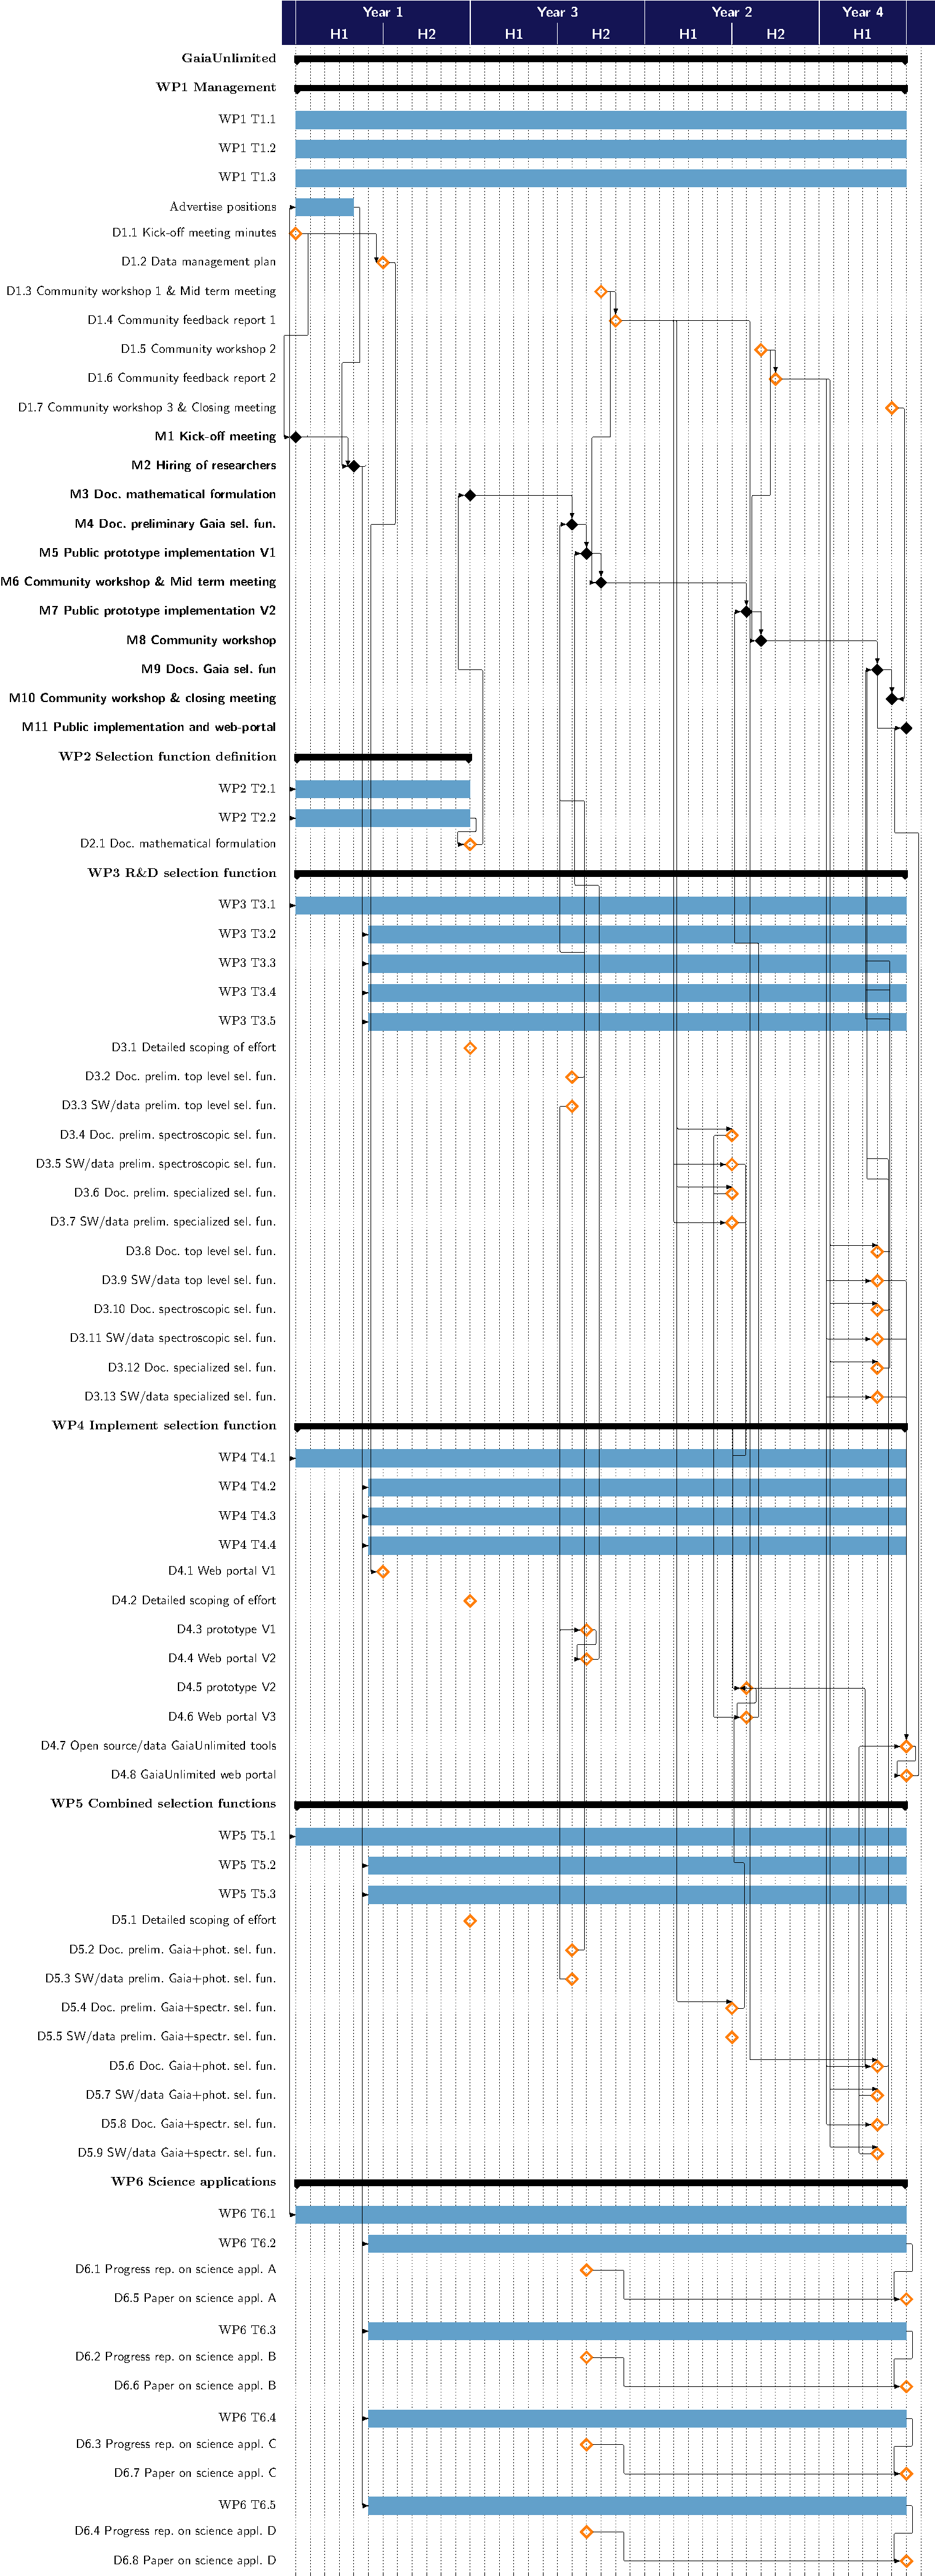
\includegraphics[height=0.95\textheight]{gaiaunlimited-gantt.pdf}
    \caption{Gantt chart for the {\acro} project.}
    \label{fig:gantt}
\end{figure}

\begin{figure}
    \centering
    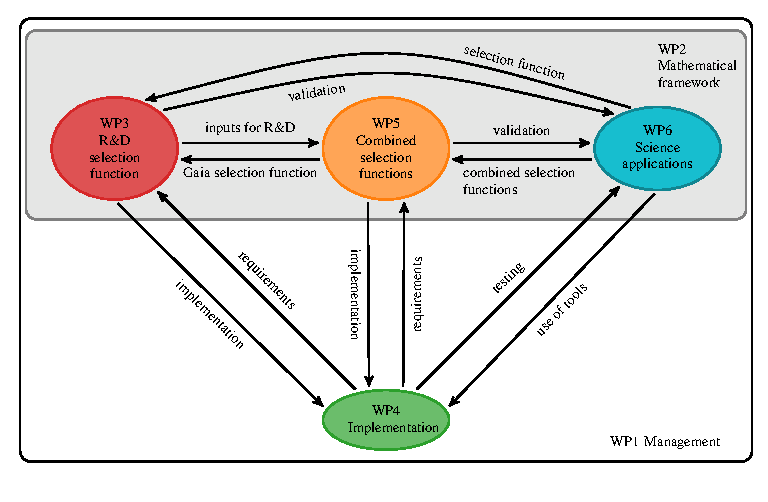
\includegraphics[width=\linewidth]{dependencies.pdf}
    \caption{The dependencies between the work packages in \acro.}
    \label{fig:dependencies}
\end{figure}

The overall approach to the work plan is to have the research and development of the selection function progress in parallel with the implementation thereof. We made this choice because of the complexities of the selection function and its realization in the form of tools and auxiliary data, and because of the relatively short duration of the project. The work flow we foresee for {\acro} is shown in \figref{fig:workflow}. It is an iterative workflow in which the findings in each of the work packages \ref{wp:selfungaia}--\ref{wp:scienceappl} will inform the others (see \figref{fig:dependencies}). For example the research on the selection function will lead to requirements on the implementation, while at the same time the conversion of research ideas into practical tools will lead to the questioning and revision of those same ideas.

At several points during the project the results will be combined into prototype implementations of the selection function tools. These will be tested both internally to the project and through the public availability of two prototype implementations. Specifically, we plan to organize two community workshops just after the public release of the prototypes to train members from the astronomical community in the use of the tools and to collect user feedback. The results from these tests will feed into the next round of research, development, and implementation. The scientific nature of much of the work conducted in {\acro} will very much benefit from an iterative approach. Close coordination between the work packages will of course be essential and this is foreseen in the management structure.

\subsection{Timing of the work packages}
\label{sec:wptiming}

The overall work plan is structured as follows:
\begin{itemize}
    \item The first 6 months will be used to recruit the post-doctoral researchers to be funded from this proposal and to carry out the tasks in work package \ref{wp:selfundefinition}. Having a mathematical framework for the selection function in place early on in the project is important for guiding the research and the implementation phases.
    \item During the next three years of the project the efforts in work packages \ref{wp:selfungaia} to \ref{wp:scienceappl} will happen in parallel as illustrated in \figref{fig:workflow}. The iterative approach outline above will be used in this phase.
    \item The selection function implementation prototypes to be developed in each phase will increase in their level of detail and complexity. We explicitly foresee two public prototypes (see \figref{fig:gantt} and WP\ref{wp:selfunimplementation}), which will be presented and tested at two community workshops. Further internal prototypes are also foreseen. Initially we may chose to implement a prototype selection function that depends only on sky position and apparent magnitudes (\figref{fig:gsf_ideal}), without any consideration for observation interruptions on the spacecraft, or on-board or ground processing effects. It would then be natural to include spacecraft outages, as these events are well-documented. Depending on the level of complexity envisaged, Prototype 2 may include on board processing effects like magnitude estimates (given the input source catalogue) and telemetry effects. Prototype 2 could also include pipeline data processing interventions that occur on the ground, or how astrophysical environments would affect the observable properties (e.g., binarity, variability). The scope of each prototype will be iteratively guided by user testing, feedback, and the executive board.
 \end{itemize}

\subsection{Dependencies}
\label{sec:dependencies}

\figrefcap{fig:dependencies} shows the dependencies between the various work packages in \acro. The arrows indicate a ‘depends on’ relationship. For example WP\ref{wp:selfuncombine} depends on WP\ref{wp:selfungaia} for the details of the Gaia selection function in order to produce combined selection functions. The reverse dependency shows that studying combined selection functions will also lead to constraints on the Gaia selection function. WP\ref{wp:scienceappl} provides the science applications which depend on WPs~\ref{wp:selfungaia} and \ref{wp:selfuncombine} for the selection functions to apply and on WP\ref{wp:selfunimplementation} for the tools to do so. In return WP\ref{wp:scienceappl} provides crucial validation of the results from WPs~\ref{wp:selfungaia} and \ref{wp:selfuncombine} and extensive testing of the implementation provided by WP\ref{wp:selfunimplementation}. WP\ref{wp:selfundefinition} provides the framework for WPs \ref{wp:selfungaia}/\ref{wp:selfuncombine}/\ref{wp:scienceappl} as indicated by the grey rectangle. The management work package (WP\ref{wp:management}) ensures the overall coordination of the {\acro} effort.

\section{Management structure, milestones and procedures}
\label{sec:management}

\subsection{Management}
\label{sec:mgtdetails}

The {\acro} consortium being relatively small the management structure can be kept simple in order to make the coordination of the efforts efficient. This structure works well for the small group of highly motivated and self-driven researchers which constitute {\acro}. The management consists of three levels, reflecting the structuring of the {\acro} work packages.
\begin{description}
    \item[Administrative management] This first level concerns the administrative management of {\acro}, including financial management and reporting to the European Commission. It is carried out by the {\acro} coordinator (A.~Brown) with the support of the Leiden Observatory institute management team.
    \item[Overall project management and coordination] This second level concerns the global scientific and technical control and coordination of the project, ensuring that the tasks are properly carried out and remain on schedule, and that the objectives of {\acro} are fulfilled. It is carried out by the \textbf{{\acro} executive board}, formed by the managers of the work packages: A.~Brown, H.-W.~Rix, R.~Drimmel, and V.~Belokurov. In order to keep communications within the consortium as efficient as possible the main contacts at NYU and MONA (D.W.~Hogg and A.~Casey) will have a standing invitation to attend the executive board meetings (see below).
    \item[Work package management] The third level of management concerns the main work packages. Each WP manager has the responsibility of supervising the execution of the core tasks assigned to their host institution, the work of the partners carrying out specific parts of the tasks attached to the work package, and report to the executive board accordingly.
    
    We do not further specify the management procedures for each work package beyond the items given above, since the work in each of the work packages \ref{wp:selfundefinition} to \ref{wp:scienceappl} will be integrated in already existing and well established teams at each host institution.
\end{description}

This management structure together with the procedures described below is sufficient for a relatively small team spread over only six institutes working together closely in a scientific environment. Much of the coordination and supervision will take place through day-to-day contacts at the institutes involved and between institutes via e-mail and ad-hoc telecons. Similar structures were applied successfully to other EU-funded projects (FP7 GENIUS Collaborative project, FP7 GREAT Marie-Curie Initial Training Network) in which the {\acro} coordinator was an active participant.

\subsection{Innovation management}
\label{sec:innovationmgmt}

The aim of {\acro} is to develop and deliver a new product (the Gaia selection function and tools to apply it) to the market of astronomy researchers. The wish for a selection function for the Gaia survey has been expressed on numerous occasions, meaning that this product will readily find a large user base. In order to uncover opportunities the astronomical community will be engaged during the lifetime of {\acro} through the availability of public prototype implementations of the Gaia selection function. Two community workshops will be organized just after the release of the prototypes at which users can test the tools by applying them to their science cases. At the same time they will be asked for feedback in the form of missing features or desired improvements. Community feedback will also be obtained through presentation of {\acro} results at relevant scientific conferences.

\subsection{Procedures and reporting}
\label{sec:procedures}

We list here the procedures that will apply to the management of {\acro}:
\begin{itemize}
    \item The {\acro} coordinator will report to the European Commission following the rules applicable for research and innovation projects within the Horizon 2020 programme.
    \item {\acro} will hold at least three plenary meetings open to participation of all its members: the kick-off, mid-term, and closing meeting. The participation of the partner institute coordinators (or a representative) will be mandatory. Other plenary meetings may be held if needed.
    \item Three community workshops will be organized which will be held in parallel to the plenary meetings. These meetings will be the occasion to train the community in the use of {\acro} tools and to have the users test the tools through using them.
    \item The executive board will hold teleconferences at least once a month to track the status of the tasks. The minutes of these teleconferences will be made available to the members of the consortium.
    \item The executive board shall ensure the coordination of the {\acro} work with the wider activities on the Gaia mission and its data releases, in particular ensuring the coordination with ESA and DPAC (see \secref{sec:dissemination-exploitation}). This can be done efficiently through membership of several {\acro} team members in DPAC.
\end{itemize}

\subsection{Consortium agreement}
\label{sec:cons_agreement}

The internal workings of {\acro} and the roles and responsibilities of the partners will be formalized through a consortium agreement which will be drawn up and agreed at the start of the programme. It will define the decision taking procedures in {\acro} and the mechanisms for conflict resolution, which will be channelled through the Executive Board, as well as the management of intellectual property rights as described in \secref{sec:dissemination-exploitation} and \secref{sec:innovationmgmt} above.

\subsection{Recruitment strategy}
\label{sec:recruit}

The recruitment policy for {\acro} will conform to the principles of the European Charter for Researchers and the Code of Conduct for their recruitment. It will take place in a globally coordinated way during the six-month setup phase described in \secref{sec:wptiming}, placing an emphasis on individual excellence and capacity for team working, while taking care to ensure equal opportunity and gender balance. The recruitment strategy will be in line with institutional practices, where each of the partner institutes has equal opportunity and gender policies in place.


\section{Consortium as a whole}
\label{sec:consortium}

The idea for this proposal grew out of discussions at several Gaia Sprints\footnote{\url{http://gaia.lol}} in which all of the {\acro} members participated, Hogg, Casey, Price-Whelan, and Rix being members of the organizing team of the Sprints. In particular at the Gaia Sprint that took place in Santa Barbara (USA) in March 2019, two sessions were dedicated solely to discussing the Gaia selection function. It was concluded that only a significant and dedicated effort, specifically funded, could realistically lead to the construction of the Gaia selection function and the corresponding tools and data needed to use it.

The consortium represents a combination of Gaia/DPAC experts (Brown, Drimmel, Fouesneau) and experts that have given much thought to the principles of selections functions and worked on aspects of the Gaia selection function (Hogg, Rix, Drimmel, Price-Whelan, Casey, Fouesneau, Belokurov, Everall). All the participants have undertaken scientific analyses of the Gaia data that clearly highlight the need for a selection function \citep[e.g.,][]{Eilers2019a,ElBadry2019,ApwGD12018}.
\begin{itemize}
    \item The Gaia expertise in the consortium is contributed by long-standing DPAC members who are deeply involved in the data processing for the Gaia mission. They provide expert insight into the detailed ingredients of the Gaia selection function and, more importantly, have an extensive network of contacts with experts in DPAC who can provide more detailed information where needed. The presence of the Gaia experts is crucial to the guidance of the researchers to be funded through {\acro}. We note that the other participants have extensive experience as users of Gaia data and thus bring an important complementary perspective to {\acro}.
    \item The expertise on the mathematical formulation of the selection function and on selection functions in general is essential to the success of {\acro}. The expertise stems from the actual construction of selection functions and applying these to analyses of a number of large surveys \citep[e.g.,][]{2012ApJ...753..148B, ElBadry2019, Eilers2019a, EverallDas2020}.
    \item The requirements on a selection function and how it is provided in its practical form must be guided by the experience gained through advanced scientific analyses of data such as from the Gaia mission. The experience from successes and failures in past analyses will be very important in setting the priorities for the research and development in {\acro}. The participants of this proposal provide the required expertise.
    \item The partners from Australia and the USA contribute deep knowledge of selection function issues based on their past scientific work. Their perspective as experienced users of the Gaia data will be essential to ensure that the developments in {\acro} stay focused on satisfying the needs of the astronomical community in general, and not just the needs of DPAC experts.
\end{itemize}

As mentioned in \secref{sec:concept} community efforts to produce (parts of) the Gaia selection function are already underway, such as the works by Boubert \& Everall \cite{Boubert2020a, Boubert2020b}\footnote{\url{https://github.com/DouglasBoubert/selectionfunctions}} and Rybizki, Drimmel \& Carrasco\footnote{\url{https://github.com/jan-rybizki/gdr2_completeness}}. Everall and Drimmel are participants in this proposal and we will work closely with D.~Boubert (Oxford) and will thus benefit from his expertise built up with concrete research into the Gaia selection function, as well as from his expertise in creating user tools.

The participants in {\acro} have a long track record of effective collaboration as can be seen from the many joint publications. Through the organization of Gaia Sprints and other workshops\footnote{For example the Gaia DR2 Exploration Lab \url{https://www.cosmos.esa.int/web/gaia-dr2-exploration}.} the participants have a proven track record of engaging the astronomical community, an important aspect of making sure that the tools and data delivered by {\acro} fulfil actual user needs.

The coordinator, A.~Brown, is also a member of the management committee of the COST action CA18104 `Revealing the Milky Way with Gaia'\footnote{\url{http://www.mw-gaia.org/}} and is co-I on the recently submitted proposal for a Marie Sk\l{}odowska-Curie Innovative Training Network also called `Revealing the Milky Way with Gaia'. We foresee participation in the conferences organized through the MW-Gaia COST action as part of the dissemination activities and if the ITN proposal is successful we would offer training in the use of the Gaia selection function to the PhD students in that network. This could take place for example at one of the schools planned by the ITN, or through participation of the PhD students in our planned community workshops (deliverables \ref{dev:wp1midtterm}, \ref{dev:wp1community}, \ref{dev:wp1closing}).

\section{Resources to be committed}
\label{sec:resources}

The person-month distribution for the {\acro} effort is shown in the summary of effort table. The workload is concentrated mostly in WPs \ref{wp:selfungaia}--\ref{wp:scienceappl}, reflecting that in those work packages the bulk of the work will be carried out by the researchers to be hired through {\acro} funding. The larger number of {\pems} assigned to MPIA reflects that combining catalogues and generating the corresponding selection functions carries the significant overhead of handling and matching multiple large catalogues.

We summarize how we arrived at the project financial budget:
\begin{itemize}
    \item Full salary costs are included for all researchers to be hired, which amounts to a total of 156 {\pems} at the rates corresponding to the institute at which they will be employed.
    \item At each of ULEI, MPIA, INAF, and UCAM one researcher at the post-doctoral level will be hired for 36 {\pems}. At MPIA an additional researcher will be hired for 12 {\pems}, at the MSc or post-doctoral level, to work on tasks \ref{task:wp4layers} and \ref{task:wp4combine}.
    \item Full salary costs are included for the participants from the staff at ULEI, INAF, and UCAM (Brown, Drimmel, Belokurov).
    \item Salary costs for the staff from MPIA, MONA, and NYU are listed but treated as in kind contributions, \emph{no EU funds are requested for these salary costs}. This explains the zero budget request for MONA and NYU.
    \item Travel costs are calculated as follows:
    \begin{itemize}
        \item For the staff at ULEI, MPIA, INAF, UCAM we estimate 1 trip in Europe per half year (7 trips total), budgeted at 1250 Euro each, and one trip to the USA, and one to Australia, both budgeted at 2500 Euro.
        \item For the researchers hired at ULEI, MPIA, INAF, UCAM we estimate 1 trip in Europe per half year (6 trips total, with 2 extra trips at MPIA reflecting the extra 12 \pems), budgeted at 1250 Euro each, and one trip to the USA, and one to Australia, both budgeted at 2500 Euro.
        \item A budget for visitors is included for each institute which will allow for a visit by the NYU and MONA partners to each of the European institutes over the lifetime of the project (each trip at 2500 Euro). Each European institute was assigned an additional 2500 Euro to accommodate for visitors from within Europe.
    \end{itemize}
    \item Equipment costs are estimated at 5500 Euro each for ULEI, MPIA, INAF, and UCAM. This allows for the provision of high end laptops and PCs to the researchers which is a necessity for this data and compute intensive project.
    \item ULEI, MPIA, INAF, and UCAM all have budgets for other goods and services. These include publication costs, and audit costs where mandatory, as detailed below.
    %\item Each of ULEI, MPIA, INAF, and UCAM are assigned a publication budget of 3000 Euro.
    \item At ULEI \EUR\ $10\,000$ is reserved for support of the workshops and setting up a web portal. In addition \EUR\ $10\,000$ is reserved for auditing costs.
\end{itemize}

For completeness the tables below contain the justifications for the partners ULEI, MPIA, INAF, and UCAM.
\medskip

\costsTravel{ULEI}{47250}{The travel costs are calculated as explained above which leads to \EUR~$33\,750$, to which \EUR~$13\,500$ is added for an extended (6 month) visit to the work with the partner at MONA (task \ref{task:wp4combine}).}
\costsEquipment{ULEI}{5500}{As explained above.}
\costsOther{ULEI}{23000}{Includes publication, auditing, workshop, and web portal costs.}

\costsTravel{MPIA}{36250}{The travel costs are calculated as explained above where the additional 12 months effort by a researcher at MPIA to be funded through {\acro} are included.}
\costsEquipment{MPIA}{5500}{As explained above.}
\costsOther{MPIA}{3000}{Publication and audit costs as explained above.}

\costsTravel{INAF}{33750}{The travel costs are calculated as explained above.}
\costsEquipment{INAF}{5500}{As explained above.}
\costsOther{INAF}{3000}{Publication costs as explained above.}

\costsTravel{UCAM}{33750}{The travel costs are calculated as explained above.}
\costsEquipment{UCAM}{5500}{As explained above.}
\costsOther{UCAM}{3000}{Publication and audit costs as explained above.}

\makecoststable

%%% Local Variables:
%%% mode: latex
%%% TeX-master: "proposal-main"
%%% End:
